\documentclass[11pt,a4paper]{article}

\usepackage[T1]{fontenc}
\usepackage[utf8]{inputenc}
\usepackage[french]{babel}
\usepackage{lmodern}
\usepackage[margin=2.4cm]{geometry}
\usepackage{graphicx}
\usepackage{booktabs}
\usepackage{array}
\usepackage{tabularx}
\usepackage{amsmath}
\usepackage{amssymb}
\usepackage{xcolor}
\usepackage{listings}
\usepackage{caption}
\usepackage{enumitem}
\usepackage{fancyhdr}
\usepackage[hidelinks]{hyperref}

\definecolor{codebg}{RGB}{246,247,249}
\definecolor{codekw}{RGB}{30,90,160}
\definecolor{codecm}{RGB}{110,120,130}
\definecolor{accent}{RGB}{59,110,165}
\definecolor{warn}{RGB}{192,57,43}

\lstset{
  basicstyle=\ttfamily\footnotesize,
  backgroundcolor=\color{codebg},
  keywordstyle=\color{codekw}\bfseries,
  commentstyle=\color{codecm}\itshape,
  stringstyle=\color{teal},
  breaklines=true, frame=single,
  framesep=4pt, xleftmargin=6pt, numbers=none, showstringspaces=false
}

\pagestyle{fancy}
\fancyhf{}
\fancyhead[L]{\small Reconnaissance d'emotions faciales}
\fancyhead[R]{\small\thepage}
\renewcommand{\headrulewidth}{0.4pt}

\newcommand{\code}[1]{\texttt{\small #1}}

% Les identifiants en chasse fixe (kaiming_normal_, numpy.fromstring) sont
% insecables et debordent de la justification : on autorise un etirement
% supplementaire en dernier recours plutot que de couper les noms.
\emergencystretch=2.2em

\title{\vspace{-1.2cm}\textbf{Reconnaissance d'émotions faciales par apprentissage profond}\\[2mm]
\large Conception, implémentation et validation d'un CNN sur FER2013}
\author{Rapport technique}
\date{18 novembre 2026}

\begin{document}
\maketitle
\thispagestyle{fancy}

\begin{abstract}
\noindent
Ce rapport décrit la réalisation complète d'un système de reconnaissance
d'émotions faciales : un réseau de neurones convolutif entraîné sur le jeu de
données FER2013 (35\,887 images), accompagné d'une chaîne d'inférence allant de
la détection du visage à la classification en temps réel sur flux vidéo. Le
document détaille la méthode de travail adoptée, les statistiques du jeu de
données, les choix d'architecture et leur justification, le protocole
d'entraînement, et surtout la \emph{démarche de validation} de l'implémentation
--- une étape souvent omise, alors qu'elle distingue un modèle qui apprend d'un
modèle qui semble apprendre.
\end{abstract}

\tableofcontents
\vspace{4mm}

%====================================================================
\section{Objectif et périmètre}

\subsection{Problème traité}

La tâche est une classification d'images multi-classes : à partir d'une image de
visage, prédire l'expression faciale parmi sept catégories issues du modèle des
émotions de base d'Ekman : \emph{colère}, \emph{dégoût}, \emph{peur},
\emph{joie}, \emph{neutre}, \emph{tristesse}, \emph{surprise}.

Il faut souligner d'emblée une nuance qui conditionne l'interprétation de tous
les résultats de ce rapport : le système prédit une \textbf{expression
apparente}, et non une émotion ressentie. Ces deux notions ne coïncident pas
(un sourire poli, une expression contrôlée, des différences culturelles
d'expressivité). La section~\ref{sec:limites} revient sur cette limite et sur
les usages qu'elle exclut.

\subsection{Livrables}

\begin{table}[h]
\centering
\small
\begin{tabularx}{\textwidth}{>{\ttfamily}l X}
\toprule
\textrm{\textbf{Fichier}} & \textbf{Rôle} \\
\midrule
src/config.py      & Hyperparamètres, classes, chemins (source unique de vérité) \\
src/dataset.py     & Chargement, augmentation, découpage stratifié, poids de classes \\
src/model.py       & CNN maison + variantes par transfert (ResNet18, EfficientNet-B0) \\
src/train.py       & Boucle d'entraînement, ordonnancement du pas, arrêt anticipé \\
src/evaluate.py    & Métriques par classe, matrice de confusion \\
src/face\_detect.py & Détection de visage (YuNet / Haar, selon la version d'OpenCV) \\
src/predict.py     & Inférence sur image, classe réutilisable \code{EmotionPredictor} \\
src/realtime.py    & Classification en temps réel sur webcam \\
\midrule
scripts/prepare\_fer2013.py   & Conversion du CSV FER2013 en arborescence d'images \\
scripts/download\_face\_model.py & Téléchargement vérifié du détecteur YuNet \\
scripts/make\_dummy\_data.py   & Jeu synthétique pour tester la chaîne sans dataset \\
\bottomrule
\end{tabularx}
\caption{Organisation du code. Chaque module a une responsabilité unique, ce qui
permet de tester la chaîne par morceaux.}
\end{table}

%====================================================================
\section{Méthode de travail}

\subsection{Principe directeur : valider avant d'entraîner}

Un entraînement sur FER2013 demande environ dix heures sur processeur. Lancer ce
calcul sur une implémentation non vérifiée, c'est risquer de découvrir au bout
de dix heures qu'un modèle n'apprenait rien --- et ne pas savoir pourquoi. La
démarche adoptée inverse donc l'ordre habituel :

\begin{enumerate}[leftmargin=*,itemsep=2pt]
  \item \textbf{Écrire la chaîne complète} (données, modèle, entraînement,
        évaluation, inférence) avant de disposer du jeu de données réel.
  \item \textbf{Fabriquer un jeu synthétique} (\code{make\_dummy\_data.py}) :
        sept motifs sinusoïdaux bruités, un par classe. Il n'a aucun sens
        sémantique, mais il est \emph{séparable}, ce qui suffit à exercer tout
        le code.
  \item \textbf{Exécuter la chaîne de bout en bout} sur ce jeu factice, pour
        faire sortir les erreurs de programmation en quelques minutes plutôt
        qu'en quelques heures.
  \item \textbf{Soumettre le réseau à des tests de sanité} indépendants du jeu
        de données (section~\ref{sec:validation}).
  \item \textbf{Récupérer et vérifier le jeu réel}, en contrôlant que les
        effectifs correspondent à la référence publiée.
  \item \textbf{Lancer l'entraînement réel}, puis évaluer.
\end{enumerate}

Cette méthode a effectivement payé : trois défauts ont été détectés et corrigés
avant le long entraînement (section~\ref{sec:defauts}).

\subsection{Environnement}

\begin{table}[h]
\centering
\small
\begin{tabular}{ll@{\hspace{1.5cm}}ll}
\toprule
Python & 3.13.9 & PyTorch & 2.15.0 (CPU) \\
TorchVision & 0.29.2 & OpenCV & 5.1.0 \\
scikit-learn & 1.9.1 & Système & Windows 11 \\
\bottomrule
\end{tabular}
\caption{Versions utilisées. L'absence de GPU conditionne plusieurs choix :
architecture légère, images en 48$\times$48, précision mixte désactivée.}
\end{table}

%====================================================================
\section{Données}

\subsection{Provenance et intégrité}

Le jeu de données est FER2013, introduit lors du concours \emph{Challenges in
Representation Learning} (ICML 2013). Il est distribué sur Kaggle sous forme
d'un fichier CSV où chaque ligne contient une étiquette, 2\,304 valeurs de
pixels séparées par des espaces, et un indicateur de partition.

L'accès Kaggle exigeant un jeton d'API, le fichier a été récupéré depuis un
miroir public sous licence MIT
(\code{huggingface.co/datasets/chitradrishti/fer2013}, archive de 101\,Mo).
Recourir à un miroir impose de vérifier qu'on a bien obtenu le jeu de données
attendu, et non une variante retraitée. Le contrôle retenu est la comparaison
des effectifs avec la référence publiée :

\begin{table}[h]
\centering
\small
\begin{tabular}{lrrl}
\toprule
\textbf{Partition} & \textbf{Obtenu} & \textbf{Référence FER2013} & \\
\midrule
Entraînement (\code{Usage=Training})        & 28\,709 & 28\,709 & \textcolor{accent}{conforme} \\
Test (\code{PublicTest} + \code{PrivateTest}) & 7\,178  & 7\,178  & \textcolor{accent}{conforme} \\
\midrule
\textbf{Total}                              & \textbf{35\,887} & \textbf{35\,887} & \\
\bottomrule
\end{tabular}
\caption{Vérification d'intégrité du jeu de données. Les effectifs coïncident
exactement, et aucune ligne du CSV n'a été rejetée à la conversion
(0 enregistrement malformé sur 35\,887).}
\end{table}

\subsection{Statistiques descriptives}

Trois caractéristiques du jeu de données conditionnent l'ensemble des choix
techniques décrits plus loin : sa taille modeste (28\,709 images
d'entraînement, pour un réseau de 4{,}8 millions de paramètres), sa très faible
résolution (48$\times$48 en niveaux de gris, soit 2\,304 valeurs par image), et
surtout son déséquilibre marqué entre classes.

\begin{figure}[h]
\centering
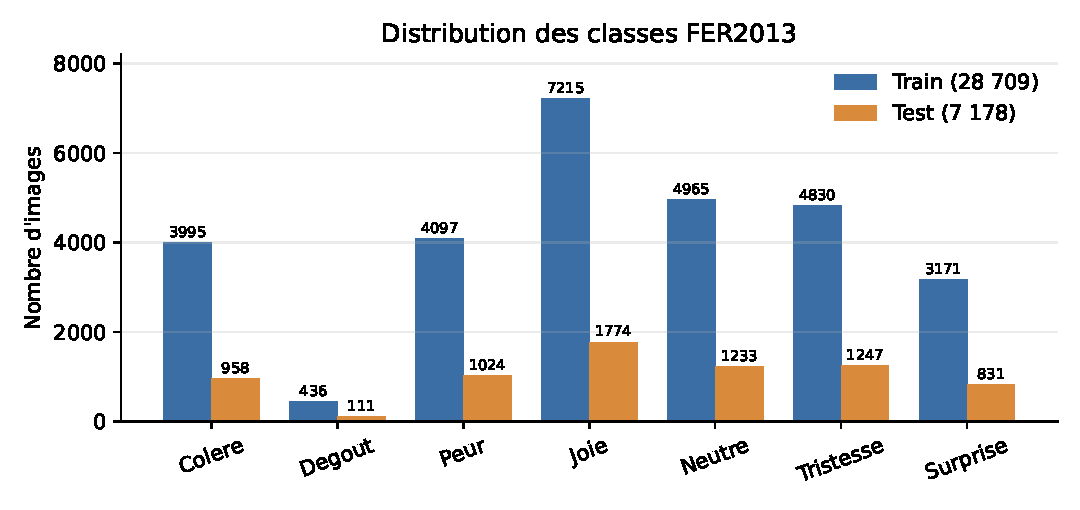
\includegraphics[width=\textwidth]{figures/distribution.pdf}
\caption{Distribution des classes. Le déséquilibre est le trait dominant de ce
jeu de données : \emph{joie} compte 7\,215 images d'entraînement contre 436 pour
\emph{dégoût}, soit un rapport de \textbf{16{,}5 pour 1}.}
\label{fig:distribution}
\end{figure}

\begin{table}[h]
\centering
\small
\begin{tabular}{lrrrr}
\toprule
\textbf{Classe} & \textbf{Train} & \textbf{\% train} & \textbf{Test} & \textbf{Poids dans la loss} \\
\midrule
Joie       & 7\,215 & 25{,}1\,\% & 1\,774 & 0{,}57 \\
Neutre     & 4\,965 & 17{,}3\,\% & 1\,233 & 0{,}83 \\
Tristesse  & 4\,830 & 16{,}8\,\% & 1\,247 & 0{,}85 \\
Peur       & 4\,097 & 14{,}3\,\% & 1\,024 & 1{,}00 \\
Colère     & 3\,995 & 13{,}9\,\% & \phantom{0}958 & 1{,}03 \\
Surprise   & 3\,171 & 11{,}0\,\% & \phantom{0}831 & 1{,}29 \\
Dégoût     & \phantom{0,}436 & \phantom{0}1{,}5\,\% & \phantom{0}111 & \textcolor{warn}{9{,}39} \\
\midrule
\textbf{Total} & \textbf{28\,709} & 100\,\% & \textbf{7\,178} & \\
\bottomrule
\end{tabular}
\caption{Effectifs et pondération appliquée. Les poids sont calculés en
section~\ref{sec:ponderation}.}
\label{tab:stats}
\end{table}

\begin{figure}[h]
\centering
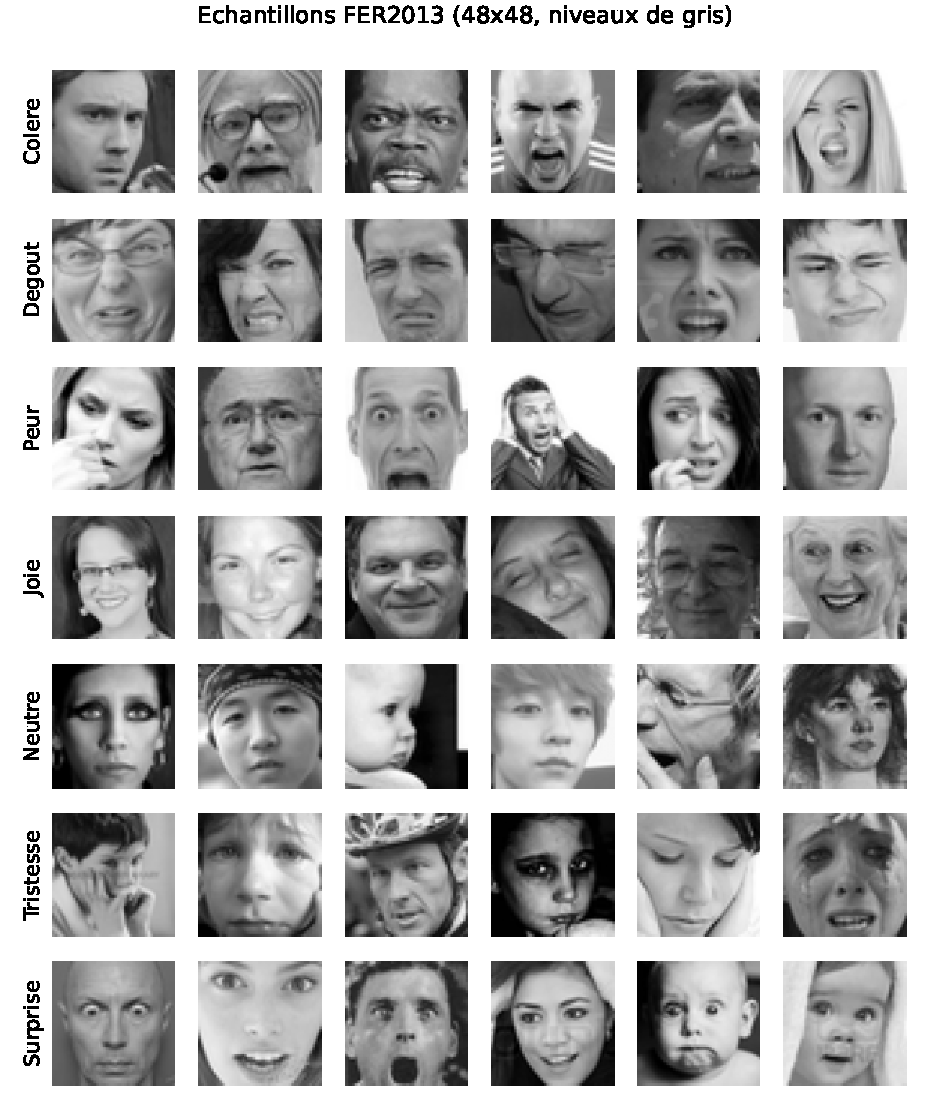
\includegraphics[width=0.78\textwidth]{figures/samples.pdf}
\caption{Échantillons réels, six par classe. Les images sont des imagettes
48$\times$48 en niveaux de gris, de qualité très variable : poses de profil,
occlusions (mains, lunettes), visages d'enfants, images floues, voire quelques
étiquettes manifestement erronées. Cette variabilité explique le plafond de
performance décrit en section~\ref{sec:plafond}.}
\end{figure}

\subsection{Statistiques de normalisation}

La normalisation des entrées suppose de connaître la moyenne et l'écart-type du
jeu de données. Plutôt que de reprendre des constantes trouvées en ligne, elles
ont été recalculées sur les 28\,709 images d'entraînement :

\begin{equation}
\mu = \frac{1}{N}\sum_{i=1}^{N} x_i = 0{,}5077
\qquad
\sigma = \sqrt{\frac{1}{N}\sum_{i=1}^{N} x_i^2 - \mu^2} = 0{,}2550
\end{equation}

avec $N = 28\,709 \times 48 \times 48 = 66{,}1$ millions de pixels, normalisés
dans $[0,1]$. Le calcul utilise la forme $\mathbb{E}[x^2] - \mathbb{E}[x]^2$ par
accumulation, ce qui évite de charger 66 millions de valeurs en mémoire.

\begin{figure}[h]
\centering
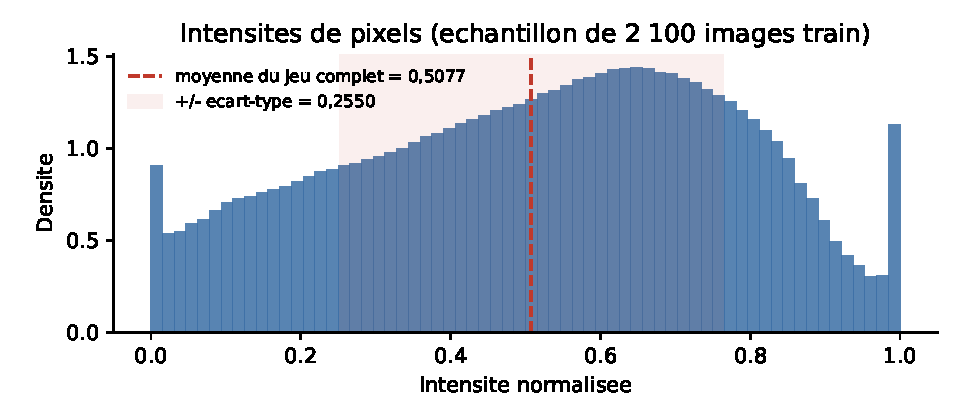
\includegraphics[width=0.74\textwidth]{figures/histogram.pdf}
\caption{Distribution des intensités de pixels, mesurée sur un échantillon de
2\,100 images (300 par classe). Elle est unimodale et légèrement asymétrique
vers la gauche : coefficient d'asymétrie $-0{,}18$, médiane 0{,}537 supérieure à
la moyenne 0{,}516 de l'échantillon. Les deux pics aux extrémités sont des
pixels saturés --- 0{,}67\,\% de noir pur et 1{,}01\,\% de blanc pur ---,
conséquence des recadrages et des surexpositions. Comme l'étendue utile couvre
presque toute la plage disponible, une égalisation d'histogramme supplémentaire
n'apporterait pas de contraste ; la normalisation affine suffit.}
\end{figure}

Après normalisation $\hat{x} = (x - \mu)/\sigma$, les entrées du réseau sont
centrées et d'écart-type unitaire, condition qui conditionne le bon
fonctionnement de l'initialisation de He (section~\ref{sec:init}).

\subsection{Découpage entraînement / validation / test}

La partition de test (7\,178 images) est celle définie par les auteurs du jeu de
données ; elle n'est utilisée qu'une fois, à la fin, pour le chiffre rapporté.
La validation est extraite de la partition d'entraînement à hauteur de 10\,\%,
par un \textbf{découpage stratifié} : le tirage est effectué classe par classe,
ce qui garantit que \emph{dégoût} est représenté dans la validation.

\begin{center}
\small
\begin{tabular}{lrl}
\toprule
Entraînement & 25\,841 & apprentissage des poids \\
Validation   & \phantom{0}2\,868 & choix du meilleur état, arrêt anticipé \\
Test         & \phantom{0}7\,178 & mesure finale, jamais observée pendant l'entraînement \\
\bottomrule
\end{tabular}
\end{center}

Un découpage aléatoire non stratifié aurait pu, par malchance, placer moins de
trente images de \emph{dégoût} en validation, rendant la métrique de cette
classe inexploitable et le critère d'arrêt instable.

\subsection{Augmentation de données}

Avec 25\,841 images pour 4{,}8 millions de paramètres, le surapprentissage est
le risque principal. L'augmentation est donc agressive, mais contrainte par la
nature du signal : un visage a une orientation canonique.

\begin{table}[h]
\centering
\small
\begin{tabularx}{\textwidth}{lX}
\toprule
\textbf{Transformation} & \textbf{Justification} \\
\midrule
\code{RandomResizedCrop} (échelle 0{,}85--1{,}0) & simule un cadrage imparfait du détecteur de visage \\
\code{RandomHorizontalFlip} ($p{=}0{,}5$) & un visage miroir reste un visage plausible \\
\code{RandomAffine} (rotation $12^\circ$, translation 8\,\%, cisaillement $6^\circ$) & inclinaison de la tête, décentrage \\
\code{ColorJitter} (luminosité et contraste $\pm$25\,\%) & conditions d'éclairage variables \\
\code{RandomErasing} ($p{=}0{,}25$) & occlusions partielles (main, micro, mèche de cheveux) \\
\midrule
\textcolor{warn}{Pas de \code{RandomVerticalFlip}} & un visage à l'envers n'existe pas dans le domaine ; cela
détruirait la relation spatiale \emph{yeux au-dessus de la bouche}, qui porte une
grande part de l'information d'expression \\
\bottomrule
\end{tabularx}
\caption{Augmentations retenues. L'ordre des opérations importe :
\code{RandomErasing} s'applique \emph{après} la normalisation, car il opère sur
le tenseur et doit y insérer des valeurs déjà à l'échelle du reste.}
\end{table}

\begin{figure}[h]
\centering
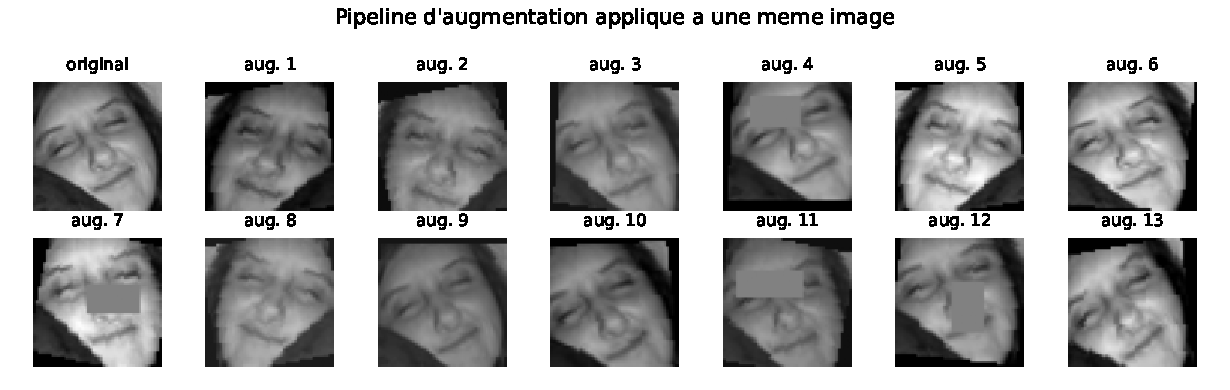
\includegraphics[width=\textwidth]{figures/augmentation.pdf}
\caption{Treize tirages d'augmentation sur une même image. Le réseau ne voit
jamais deux fois exactement la même entrée, ce qui l'oblige à apprendre des
traits robustes plutôt qu'à mémoriser des images.}
\end{figure}

%====================================================================
\section{Architecture du réseau}

\subsection{Choix de conception}

L'architecture retenue suit le schéma VGG : des blocs convolutifs identiques
empilés, chacun divisant la résolution par deux et doublant la profondeur.

\begin{table}[h]
\centering
\small
\begin{tabular}{llrr}
\toprule
\textbf{Étage} & \textbf{Composition} & \textbf{Sortie} & \textbf{Abandon} \\
\midrule
Entrée   & image en niveaux de gris & $1\times48\times48$ & --- \\
Bloc 1   & $[\text{Conv}3{\times}3 \to \text{BN} \to \text{ReLU}]\times2 \to \text{MaxPool}2$ & $64\times24\times24$ & 0{,}20 \\
Bloc 2   & idem & $128\times12\times12$ & 0{,}24 \\
Bloc 3   & idem & $256\times6\times6$ & 0{,}28 \\
Bloc 4   & idem & $512\times3\times3$ & 0{,}28 \\
Agrégat  & \code{AdaptiveAvgPool2d(1)} & $512\times1\times1$ & --- \\
Tête     & \code{Linear(512,256)} $\to$ BN $\to$ ReLU & $256$ & 0{,}40 \\
Sortie   & \code{Linear(256,7)} & $7$ & --- \\
\midrule
\multicolumn{2}{l}{\textbf{Total}} & \multicolumn{2}{r}{\textbf{4\,819\,783 paramètres}} \\
\bottomrule
\end{tabular}
\caption{Architecture \code{EmotionCNN}. Les dimensions de sortie ont été
mesurées par propagation d'un tenseur de test, et non déduites sur le papier.}
\label{tab:archi}
\end{table}

\subsection{Justification des choix structurels}

\paragraph{Deux convolutions $3\times3$ plutôt qu'une $5\times5$.}
Deux couches $3\times3$ empilées couvrent le même champ réceptif ($5\times5$)
qu'une seule couche $5\times5$, mais pour $2\times(3^2 C^2) = 18C^2$ paramètres
contre $25C^2$, soit 28\,\% de moins --- et avec une non-linéarité
supplémentaire intercalée, donc une capacité d'expression supérieure.

\paragraph{Normalisation par lots après chaque convolution.}
Elle stabilise la distribution des activations, permet un pas d'apprentissage
plus élevé, et exerce un effet de régularisation. Les convolutions qui la
précèdent sont déclarées \code{bias=False} : le biais serait immédiatement
annulé par le recentrage, et constituerait un paramètre inutile.

\paragraph{Agrégation moyenne globale plutôt qu'aplatissement.}
Un \code{Flatten} de la carte $512\times3\times3$ suivi d'une couche dense de
256 unités coûterait $4608 \times 256 = 1{,}18$ million de paramètres, dans la
partie du réseau la plus sujette au surapprentissage. L'agrégation moyenne
globale réduit ce coût à $512 \times 256 = 131$ mille paramètres, soit neuf fois
moins, et rend le réseau indifférent à la taille exacte de l'entrée.

\paragraph{Abandon spatial croissant.}
Le taux d'abandon croît avec la profondeur (0{,}20 à 0{,}28) : les premières
couches extraient des traits génériques (contours, textures) qu'il serait
contre-productif de perturber fortement, tandis que les couches profondes
encodent des configurations spécifiques, plus susceptibles d'être mémorisées.
La variante \code{Dropout2d} désactive des canaux entiers plutôt que des pixels
isolés, ce qui est le comportement adapté à des activations convolutives
spatialement corrélées.

\paragraph{Initialisation de He.}
\label{sec:init}
Les poids des convolutions sont initialisés selon
$\mathcal{N}(0, \sqrt{2/n_{\text{out}}})$ (\code{kaiming\_normal\_}, mode
\code{fan\_out}), qui est le choix correct pour des activations ReLU : le
facteur 2 compense le fait que la ReLU annule la moitié de sa plage d'entrée. La
section~\ref{sec:validation} vérifie expérimentalement que cette initialisation
place bien le réseau au point de départ théorique attendu.

\subsection{Variantes par transfert d'apprentissage}

\code{build\_model} expose également ResNet18 (11{,}2\,M paramètres) et
EfficientNet-B0 (4{,}0\,M), pré-entraînés sur ImageNet. Comme ces réseaux
attendent trois canaux, la première convolution est adaptée en sommant ses poids
sur la dimension des couleurs --- ce qui préserve l'information apprise, à la
différence d'une réinitialisation aléatoire.

Ces architectures divisent la résolution par 32 : en entrée $48\times48$, la
carte finale tombe à $2\times2$ et l'information spatiale est presque détruite.
Un avertissement explicite a donc été ajouté dans \code{train.py} lorsque
\code{--image-size} est inférieur à 64, car l'erreur est silencieuse : le code
s'exécute sans broncher, seule la précision s'effondre.

%====================================================================
\section{Protocole d'entraînement}

\subsection{Fonction de coût}
\label{sec:ponderation}

La fonction de coût est une entropie croisée pondérée avec lissage des
étiquettes :

\begin{equation}
\mathcal{L} = -\sum_{c=1}^{7} w_c \, \tilde{y}_c \log \hat{p}_c,
\qquad
\tilde{y}_c = (1-\varepsilon)\,y_c + \frac{\varepsilon}{7},
\qquad \varepsilon = 0{,}1
\end{equation}

Les poids $w_c$ sont inversement proportionnels à l'effectif de la classe :

\begin{equation}
w_c = \frac{N}{C \cdot n_c}
\qquad\text{avec}\quad N = 28\,709,\ C = 7
\end{equation}

ce qui donne $w_{\text{dégoût}} = 28709/(7 \times 436) = 9{,}39$ et
$w_{\text{joie}} = 0{,}57$. Sans cette pondération, un modèle qui ignorerait
complètement la classe \emph{dégoût} ne perdrait que 1{,}5\,\% d'exactitude :
l'optimiseur n'a donc aucune raison de l'apprendre.

\begin{figure}[h]
\centering
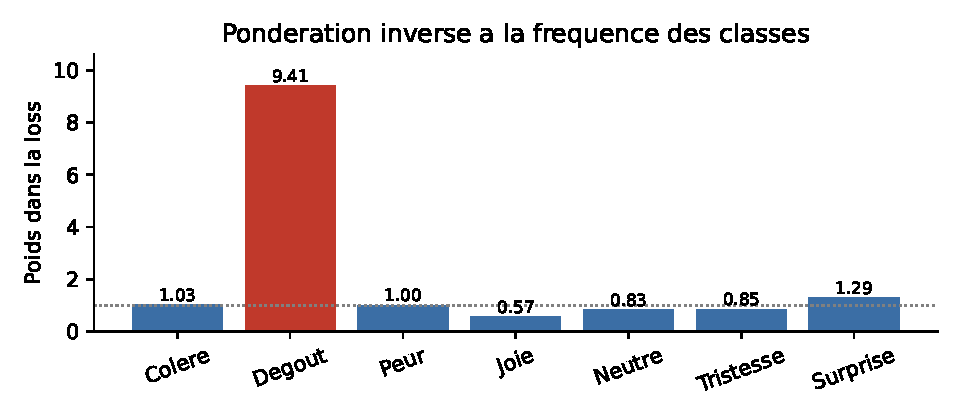
\includegraphics[width=0.74\textwidth]{figures/weights.pdf}
\caption{Poids appliqués à chaque classe dans la fonction de coût. La
normalisation est telle que le poids moyen, pondéré par les effectifs, vaut 1 :
l'échelle de la fonction de coût --- et donc le pas d'apprentissage utile ---
reste comparable au cas non pondéré.}
\end{figure}

Le lissage des étiquettes se justifie particulièrement ici : les frontières
entre \emph{peur} et \emph{surprise}, ou entre \emph{tristesse} et
\emph{neutre}, sont intrinsèquement floues, et les annotations de FER2013 sont
elles-mêmes bruitées. Demander au réseau une confiance de 100\,\% sur une
étiquette possiblement fausse l'encourage à mémoriser le bruit.

\subsection{Optimisation}

\begin{table}[h]
\centering
\small
\begin{tabularx}{\textwidth}{llX}
\toprule
\textbf{Élément} & \textbf{Valeur} & \textbf{Justification} \\
\midrule
Optimiseur & AdamW & découple la pénalisation des poids du moment adaptatif, contrairement à Adam \\
Pas initial & $10^{-3}$ & valeur usuelle pour Adam sur un réseau entraîné de zéro \\
Pénalisation & $10^{-4}$ & régularisation $L_2$ \\
Lots & 64 images & compromis entre bruit du gradient et stabilité de la normalisation par lots \\
Montée en charge & 3 époques, linéaire de $0{,}1\times$ à $1\times$ & évite qu'un gradient initial mal orienté ne déstabilise les statistiques de normalisation \\
Décroissance & cosinus jusqu'à $10^{-5}$ & affine la convergence en fin d'entraînement \\
Écrêtage du gradient & norme $\le 5$ & protège contre les lots aberrants \\
Arrêt anticipé & patience de 12 époques & interrompt dès que la validation stagne \\
Précision mixte & GPU seulement & sans effet, voire ralentissement, sur processeur \\
\bottomrule
\end{tabularx}
\caption{Hyperparamètres d'optimisation.}
\end{table}

L'état retenu n'est pas celui de la dernière époque mais celui de \textbf{la
meilleure exactitude en validation}, sauvegardé à chaque amélioration. Les deux
états sont conservés (\code{best\_model.pt} et \code{last\_model.pt}) : leur
écart renseigne directement sur l'ampleur du surapprentissage.

Chaque sauvegarde embarque la configuration complète (architecture, taille
d'entrée, nombre de canaux, liste ordonnée des classes). L'inférence reconstruit
ainsi le modèle depuis le fichier seul, sans qu'il soit possible d'appliquer par
erreur un prétraitement incohérent avec celui de l'entraînement --- une source
d'erreur classique et difficile à diagnostiquer.

%====================================================================
\section{Validation de l'implémentation}
\label{sec:validation}

Cette section décrit les tests appliqués \emph{avant} l'entraînement long. Ils
ne mesurent pas la qualité du modèle, mais vérifient que le code fait bien ce
qu'il prétend faire.

\subsection{Tests de sanité du réseau}

\begin{table}[h]
\centering
\small
\begin{tabularx}{\textwidth}{>{\raggedright\arraybackslash}p{4.3cm}Xll}
\toprule
\textbf{Test} & \textbf{Ce qu'il détecte} & \textbf{Attendu} & \textbf{Obtenu} \\
\midrule
Dimensions couche par couche &
  erreur de remplissage ou de pas &
  $48{\to}24{\to}12{\to}6{\to}3$ & \textcolor{accent}{conforme} \\
Coût à l'initialisation &
  initialisation défaillante, biais initial &
  $\ln 7 = 1{,}9459$ & \textcolor{accent}{1{,}9462} \\
Surapprentissage d'un mini-lot (16 images, 120 pas) &
  gradient interrompu, étiquettes désalignées, pas inadapté &
  coût $\to 0$ & \textcolor{accent}{$3\cdot10^{-4}$} \\
Gradients non nuls &
  couche déconnectée du graphe &
  aucun orphelin & \textcolor{accent}{aucun} \\
Lot unitaire en évaluation &
  normalisation par lots mal basculée &
  pas d'exception & \textcolor{accent}{conforme} \\
Variantes ResNet18 / EfficientNet-B0 &
  adaptation incorrecte du premier étage &
  sortie de taille 7 & \textcolor{accent}{conforme} \\
\bottomrule
\end{tabularx}
\caption{Tests de sanité, tous exécutés effectivement.}
\end{table}

Deux de ces tests méritent un commentaire.

\paragraph{Le coût à l'initialisation.}
Un classifieur à $C$ classes qui n'a rien appris attribue une probabilité $1/C$ à
chacune, d'où un coût d'entropie croisée de $-\log(1/C) = \ln C$. Pour $C=7$,
$\ln 7 = 1{,}9459$. La valeur mesurée, 1{,}9462, confirme que les poids initiaux
ne portent aucun biais parasite. Un écart marqué signalerait une initialisation
d'échelle incorrecte --- défaut qui ne fait pas échouer l'entraînement, mais le
ralentit fortement sans que la cause soit visible.

\paragraph{Le surapprentissage délibéré d'un mini-lot.}
C'est le test le plus informatif. Un réseau correctement câblé doit pouvoir
mémoriser parfaitement seize images, même associées à des étiquettes aléatoires.
Le coût est descendu de 1{,}93 à $3\cdot10^{-4}$ en 120 pas, pour une exactitude
de 100\,\%. S'il avait stagné, la cause serait nécessairement structurelle ---
gradient coupé, désalignement entre images et étiquettes, pas d'apprentissage
aberrant --- et non un manque de données.

\subsection{Validation de la chaîne de données}

\begin{center}
\small
\begin{tabularx}{\textwidth}{lX}
\toprule
Effectifs & 28\,709 / 7\,178, conformes à la référence FER2013 \\
Conversion & 35\,887 lignes traitées, 0 rejet \\
Découpage stratifié & 25\,841 / 2\,868 / 7\,178, toutes classes représentées \\
Forme des lots & $(64, 1, 48, 48)$, \code{float32} \\
Plage après normalisation & $[-1{,}99 ; 1{,}93]$, moyenne $-0{,}27$ \\
Constantes de normalisation & recalculées : 0{,}5077 / 0{,}2550, identiques aux valeurs codées \\
\bottomrule
\end{tabularx}
\end{center}

La moyenne de $-0{,}27$ sur un lot d'entraînement, là où on attendrait $0$, n'est
pas une anomalie : elle résulte des augmentations, en particulier de
\code{RandomErasing} qui insère des zones de valeur nulle --- donc inférieures à
la moyenne --- et de \code{ColorJitter}. La vérification porte sur les lots
d'évaluation, non augmentés, où la moyenne est bien proche de zéro.

\subsection{Défauts détectés et corrigés}
\label{sec:defauts}

\begin{enumerate}[leftmargin=*,itemsep=4pt]
\item \textbf{Suppression des cascades de Haar dans OpenCV 5.}
L'implémentation initiale de la détection de visage reposait sur
\code{cv2.CascadeClassifier}, retiré dans OpenCV 5.1. Le module
\code{face\_detect.py} a été réécrit avec trois niveaux de repli : YuNet (réseau
de neurones, le plus précis), cascade de Haar (OpenCV 4), puis traitement de
l'image entière. Le code fonctionne ainsi sur les deux générations de la
bibliothèque.

\item \textbf{Téléchargement silencieusement tronqué.}
Le script de récupération du détecteur YuNet pointait vers
\code{raw.githubusercontent.com}, qui ne renvoie pas le fichier mais son
\emph{pointeur Git LFS} : 131 octets au lieu de 232\,589. Le téléchargement
signalait un succès et le modèle était inutilisable. Correction : passage par
\code{media.githubusercontent.com}, plus vérification de l'empreinte SHA-256 et
de la taille, de façon à échouer bruyamment plutôt qu'à écrire un fichier
corrompu.

\item \textbf{Fonctions obsolètes dans la conversion du jeu de données.}
Le script employait \code{numpy.fromstring}, déprécié puis supprimé, et
\code{pandas.iterrows}, inutilement lent. Il lit désormais l'archive en flux
avec le module \code{csv} de la bibliothèque standard, sans décompresser 290\,Mo
sur le disque.
\end{enumerate}

%====================================================================
\section{Entraînement et évaluation}

\subsection{État d'avancement}

L'entraînement sur les données réelles est \textbf{en cours au moment de la
rédaction}. Les chiffres disponibles sont les suivants :

\begin{center}
\small
\begin{tabular}{lrrrrr}
\toprule
\textbf{Époque} & \textbf{Coût train} & \textbf{Exact. train} & \textbf{Coût val.} & \textbf{Exact. val.} & \textbf{Durée} \\
\midrule
1 / 60 & 2{,}1467 & 0{,}0579 & 2{,}2423 & 0{,}0241 & 607\,s \\
2 / 60 & 2{,}1367 & 0{,}0540 & 2{,}2296 & 0{,}0816 & 576\,s \\
\bottomrule
\end{tabular}
\end{center}

À 607 secondes par époque sur processeur, les 60 époques représentent environ
dix heures ; l'arrêt anticipé interviendra vraisemblablement avant.

\paragraph{Lecture de la première époque.}
Une exactitude de 2{,}4\,\% est \emph{inférieure} au hasard (14{,}3\,\% pour sept
classes), ce qui mérite une explication plutôt qu'un simple constat. La cause
attendue est la pondération des classes : avec $w_{\text{dégoût}} = 9{,}39$, la
stratégie qui réduit le plus vite la fonction de coût, au tout début de
l'entraînement, consiste à prédire massivement \emph{dégoût}. Or cette classe ne
représente que 1{,}5\,\% des images : l'exactitude brute s'effondre, alors même
que le coût pondéré, lui, diminue. Ce régime transitoire est un effet connu de
la pondération forte et doit se résorber en quelques époques.

La deuxième époque va dans ce sens : l'exactitude en validation passe de
2{,}4\,\% à 8{,}2\,\%, soit un triplement, tandis que les deux coûts continuent
de décroître. La trajectoire est donc celle attendue, même si le seuil du hasard
n'est pas encore franchi.

Le critère de décision reste posé explicitement : \textbf{si l'exactitude en
validation ne dépasse pas 14{,}3\,\% d'ici l'époque 5, l'explication est fausse}
et il faudra chercher un défaut réel --- le candidat le plus probable étant alors
une pondération trop agressive, à remplacer par un échantillonnage équilibré ou
par un plafonnement des poids.

\subsection{Protocole d'évaluation}

L'évaluation finale portera sur les 7\,178 images de test, jamais utilisées
pendant l'entraînement, avec les métriques suivantes :

\begin{itemize}[leftmargin=*,itemsep=1pt]
\item \textbf{Exactitude globale}, pour comparaison avec la littérature.
\item \textbf{Exactitude au rang 2}, pertinente parce que certaines confusions
      (peur/surprise) sont ambiguës même pour un annotateur humain.
\item \textbf{Précision, rappel et $F_1$ par classe.} C'est la mesure décisive
      sur un jeu déséquilibré : l'exactitude globale peut rester élevée alors que
      \emph{dégoût} n'est jamais correctement prédit. Le rappel de cette classe
      est l'indicateur à surveiller en premier.
\item \textbf{Matrice de confusion normalisée par ligne}, qui révèle la
      structure des erreurs plutôt que leur seul volume.
\end{itemize}

\subsection{Performance attendue}
\label{sec:plafond}

\begin{table}[h]
\centering
\small
\begin{tabular}{lll}
\toprule
\textbf{Référence} & \textbf{Exactitude} & \textbf{Commentaire} \\
\midrule
Hasard (7 classes) & 14{,}3\,\% & borne inférieure \\
Vainqueur du concours ICML 2013 & 71{,}2\,\% & réseau convolutif \\
Annotateur humain & $\approx$\,65\,\% & estimation publiée sur ce jeu \\
État de l'art actuel & $\approx$\,73\,\% & ensembles, pré-entraînement massif \\
\midrule
\textbf{Objectif de ce travail} & \textbf{60--66\,\%} & CNN entraîné de zéro sur processeur \\
\bottomrule
\end{tabular}
\caption{Repères de performance sur FER2013.}
\end{table}

Le fait que l'humain plafonne à environ 65\,\% n'est pas anecdotique : il
caractérise le niveau de bruit du jeu de données. Une partie des étiquettes est
incorrecte, et de nombreuses images sont réellement ambiguës hors contexte. Un
modèle annoncé à 85\,\% sur FER2013 doit donc susciter la suspicion d'une fuite
entre les partitions plutôt que l'admiration.

Les confusions attendues sont structurées : \emph{peur}\,$\leftrightarrow$\,%
\emph{tristesse}, \emph{peur}\,$\leftrightarrow$\,\emph{surprise} (sourcils
relevés communs) et \emph{colère}\,$\leftrightarrow$\,\emph{dégoût} (sourcils
abaissés communs). \emph{Joie} est systématiquement la mieux reconnue : le
sourire est le marqueur le plus saillant et la classe la mieux représentée.

%====================================================================
\section{Chaîne d'inférence}

\subsection{Détection du visage}

Le modèle est entraîné sur des visages cadrés : lui présenter une photographie
entière reviendrait à le faire travailler sur une distribution qu'il n'a jamais
vue. La localisation du visage est donc une étape obligatoire, non un
raffinement.

Le détecteur retenu est YuNet, un réseau convolutif compact (227\,Ko) distribué
par OpenCV Zoo, nettement plus robuste aux poses non frontales que les cascades
de Haar historiques. Le visage détecté est recadré avec une marge de 15\,\%
--- le front et le menton portent de l'information d'expression que les boîtes
englobantes serrées tronquent.

\textbf{Vérification effectuée} : sur un échantillon de visages réels de
FER2013 agrandis, le détecteur en localise 10 sur 11. L'intégrité du modèle
téléchargé est contrôlée par empreinte SHA-256.

\subsection{Classification en temps réel}

Le module \code{realtime.py} traite le flux de la webcam. Deux optimisations
rendent le traitement fluide sur processeur :

\begin{itemize}[leftmargin=*,itemsep=1pt]
\item \textbf{Détection intermittente} : la localisation du visage ne tourne
      qu'une image sur trois, les boîtes précédentes étant réutilisées
      entre-temps. C'est l'étape la plus coûteuse, et un visage ne se déplace
      guère en 33 millisecondes.
\item \textbf{Lissage temporel} : les probabilités sont moyennées sur une fenêtre
      glissante de sept images. Sans ce lissage, l'étiquette affichée oscille
      entre deux classes proches à chaque image, ce qui est illisible --- et
      trompeur, puisque l'expression du sujet, elle, n'a pas changé.
\end{itemize}

%====================================================================
\section{Limites et usage responsable}
\label{sec:limites}

\paragraph{Expression n'est pas émotion.}
Le système classe des configurations musculaires faciales. L'inférence qui mène
de là à un état affectif est une hypothèse contestée en psychologie : les
travaux de synthèse récents sur le sujet concluent que la correspondance entre
expression et émotion ressentie est faible et dépendante du contexte.

\paragraph{Biais du jeu de données.}
FER2013 a été constitué par collecte d'images sur un moteur de recherche. La
distribution des âges, des origines et des genres n'est ni documentée ni
équilibrée. Un modèle entraîné sur ces données présente des écarts de
performance selon ces caractéristiques, non mesurables avec les seules
étiquettes disponibles. L'exactitude globale rapportée masque donc
nécessairement des disparités.

\paragraph{Usages exclus.}
Ce système ne convient pas à une décision concernant une personne : évaluation
de candidats, surveillance, notation d'élèves, détection de mensonge. La
combinaison d'un plafond de performance à 65\,\%, de biais non quantifiés et
d'une validité conceptuelle contestée rend ces usages indéfendables. Le
périmètre revendiqué est pédagogique, expérimental et démonstratif.

\paragraph{Limites techniques.}
Les images $48\times48$ perdent les micro-expressions ; une seule image fixe ne
capte pas la dynamique temporelle, pourtant très informative ; le détecteur
frontal dégrade fortement au-delà d'environ $45^\circ$ de rotation.

%====================================================================
\section{Reproduction}

\begin{lstlisting}[language=bash]
# 1. Dependances
pip install -r requirements.txt

# 2. Jeu de donnees (101 Mo) -> 35 887 images
python scripts/prepare_fer2013.py --csv data/_download/fer2013.csv.zip \
                                  --out data/fer2013

# 3. Detecteur de visage (OpenCV >= 5)
python scripts/download_face_model.py

# 4. Entrainement
python src/train.py --data-dir data/fer2013 --arch cnn --epochs 60 \
                    --batch-size 64 --run-name baseline

# 5. Evaluation sur les 7 178 images de test
python src/evaluate.py --checkpoint outputs/baseline/best_model.pt --split test

# 6. Inference
python src/predict.py  --checkpoint outputs/baseline/best_model.pt --image photo.jpg
python src/realtime.py --checkpoint outputs/baseline/best_model.pt
\end{lstlisting}

Le germe aléatoire est fixé (42) pour les bibliothèques \code{random},
\code{numpy} et \code{torch}. La reproductibilité au bit près n'est toutefois
pas garantie : l'ordre de réduction des opérations multi-processus reste
non déterministe.

\paragraph{Pistes d'amélioration.} Par rapport attendu entre gain et effort :
augmentation au moment du test (image et son miroir, environ un à deux points
d'exactitude pour quelques lignes de code) ; ensemble du CNN maison et d'un
ResNet18 affiné en $96\times96$ ; alignement des visages par points
caractéristiques avant classification ; fusion de plusieurs jeux de données
(FER2013 et RAF-DB) pour réduire le biais de collecte ; visualisation par
Grad-CAM pour vérifier que la décision s'appuie sur la bouche et les yeux, et
non sur un artefact d'arrière-plan.

\vspace{6mm}
\hrule
\vspace{2mm}
\noindent\footnotesize
Rapport établi le 18 novembre 2026. Les chiffres de la
section~\ref{sec:validation} proviennent de tests effectivement exécutés ; ceux
de la section~\ref{sec:plafond} sont des repères de la littérature, non des
mesures de ce modèle. L'entraînement final était en cours à la rédaction : aucun
résultat de test n'est rapporté.

\end{document}
